\documentclass[class=article]{standalone}
\usepackage{tikz}
%--------------------------Main Document----------------------------%
\begin{document}
    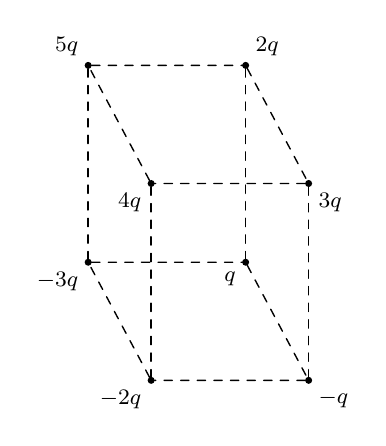
\begin{tikzpicture}[%
        line width=0.5pt,
        line cap=round,
        font=\footnotesize
    ]
        \begin{scope}[%
            every node/.style={
                circle,
                fill=black,
                draw=black,
                inner sep=0pt,
                minimum size=2pt
            }
        ]
            \node (a) at (0,0) {};
            \node (b) at (2,0) {};
            \node (c) at (2.8,-1.5) {};
            \node (d) at (0.8,-1.5) {};
            \node (e) at (0,-2.5) {};
            \node (f) at (2,-2.5) {};
            \node (g) at (2.8,-4) {};
            \node (h) at (0.8,-4) {};
        \end{scope}
        \node at (a) [above left] {$5q$};
        \node at (b) [above right] {$2q$};
        \node at (c) [below right] {$3q$};
        \node at (d) [below left] {$4q$};
        \node at (e) [below left] {$-3q$};
        \node at (f) [below left] {$q$};
        \node at (g) [below right] {$-q$};
        \node at (h) [below left] {$-2q$};
        \draw[dashed] (a) to (2,0) (b) to (c) to (d) to (a);
        \draw[dashed] (e) to (f) to (g) to (h) to (e);
        \draw[dashed] (a) to (e);
        \draw[dashed] (b) to (f);
        \draw[dashed] (c) to (g);
        \draw[dashed] (d) to (h);
    \end{tikzpicture}
\end{document}